\documentclass[11pt,letterpaper]{article}
\usepackage[T1]{fontenc}
\usepackage[utf8]{inputenc}
\usepackage{lmodern}
\usepackage[margin=1in,headheight=15pt]{geometry}
\usepackage{amsmath,amssymb,amsthm,mathtools}
\usepackage{microtype,booktabs,array,longtable,enumitem,graphicx}
\usepackage[dvipsnames]{xcolor}
\usepackage{fancyhdr,placeins}
\usepackage[unicode,colorlinks=true,linkcolor=MidnightBlue,citecolor=MidnightBlue,urlcolor=MidnightBlue]{hyperref}
\usepackage[nameinlink,noabbrev]{cleveref}
\usepackage{bookmark}
\newtheorem{theorem}{Theorem}[section]
\newtheorem{proposition}[theorem]{Proposition}
\newtheorem{lemma}[theorem]{Lemma}
\newtheorem{corollary}[theorem]{Corollary}
\theoremstyle{definition}
\newtheorem{definition}[theorem]{Definition}
\newtheorem{example}[theorem]{Example}
\theoremstyle{remark}
\newtheorem{remark}[theorem]{Remark}
\DeclareMathOperator{\Li}{Li}
\DeclareMathOperator{\Log}{Log}
\DeclareMathOperator{\Rea}{Re}
\newcommand{\eps}{\varepsilon}
\newcommand{\R}{\mathbb R}
\newcommand{\C}{\mathbb C}
\newcommand{\N}{\mathbb N}
\newcommand{\E}{\mathbb E}
\newcommand{\Prob}{\mathbb P}
\newcommand{\HH}{\mathcal H}
\newcommand{\ph}{\varphi}
\newcommand{\normal}{\mathfrak g}
\newcommand{\stir}[2]{\left\{\begin{matrix}#1\\#2\end{matrix}\right\}}
\newcommand{\pin}{\texttt{8f5afd4d7565df808359f6a0c22f87f79a119bb9}}
\pagestyle{fancy}
\fancyhf{}
\fancyhead[L]{\small Polylogarithmic coefficient transseries}
\fancyhead[R]{\small ProveIt research continuation}
\fancyfoot[C]{\thepage}
\setlength{\parskip}{4pt}
\setlength{\emergencystretch}{2em}
\renewcommand{\topfraction}{0.9}
\renewcommand{\textfraction}{0.08}
\renewcommand{\floatpagefraction}{0.85}
\setcounter{topnumber}{3}
\setlist{itemsep=3pt,topsep=5pt}
\numberwithin{equation}{section}
\hypersetup{pdftitle={Uniform coefficient transseries across the polylogarithmic order-three resonance},pdfauthor={Research continuation for the ProveIt project}}
\begin{document}
\hypersetup{pageanchor=false}
\begin{titlepage}
\centering
{\small\scshape Analysis / Polylogarithms / Transseries\par}
\vspace{1.2cm}
{\LARGE\bfseries Uniform Coefficient Transseries\par}
\vspace{0.25cm}
{\LARGE\bfseries across the Polylogarithmic\par}
\vspace{0.25cm}
{\LARGE\bfseries Order-Three Resonance\par}
\vspace{0.65cm}
{\large Exact normalization, Gaussian order derivatives,\par
Lambert transitions, and reciprocal-order inverse germs\par}
\vspace{0.9cm}
{Prepared for Vladimir Reshetnikov and the ProveIt project\par}
{12 October 2026\par}
\vspace{0.65cm}
\begin{minipage}{0.94\textwidth}
\begin{abstract}
The quadratic-feedback equation
$uv-v^2/2=\Li_s(re^v)$ has different coefficient laws below, at,
and above $s=3$. Recent repository work determines its fixed-order laws
and a joint varying-order inverse chart, but explicitly leaves the
corresponding joint coefficient problem open. We resolve that problem
when $(s-3)\log n$ remains bounded, allowing the feedback parameter to
vary simultaneously. A pole-paired scalar equation defines an exact
Gaussian scale. In that scale every inverse-logarithmic correction is
a finite Stirling-number combination of order derivatives of a
parabolic cylinder function. We prove an absolute remainder of order
$(\log n)^{-N-1}$ at every fixed order, uniformly over all lattice
locations and compact parameter sets.

At exact resonance the scale is expressed by the lower Lambert branch.
At the center the correction functions reduce to finite Gamma moments,
and reproduce the previous marginal coefficient polynomials at every
order. More generally the entire logarithmic expansion survives positive
analytic composition of the polylogarithm; the nonlinear composition
enters only through its first two endpoint derivatives after centering
and endpoint normalization. The same expansion yields relative
positive-tail matching in every fixed power-of-$\log n$ window and an
explicit Lambert location for the Gaussian--power-tail transition.

A separate local theorem classifies finite ramification of inverse
polylogarithms for every real $s>1$. The endpoint is removable precisely
at $s=1+1/m$, $m\ge2$. We give a convergent crossover chart through those
orders and prove that the integer cut-modulus argument cannot extend
to $1<s<3/2$. Complete analytic proofs, a focused source audit, exact
symbolic checks, numerical diagnostics, and further research targets
accompany the report.
\end{abstract}
\end{minipage}
\vfill
\begin{minipage}{0.94\textwidth}\small
\textbf{Scope and status.} This is an unrefereed research manuscript with
conventional proofs and reproducible checks. The results are not
proof-assistant formalized. The contribution is specified relative to
the inspected repository snapshot and the primary literature;
worldwide publication priority is not asserted. All coefficient
expansions are fixed-order asymptotic statements. The reciprocal-order
local chart has a separate, proved convergence assertion.
\end{minipage}
\end{titlepage}
\pagenumbering{roman}
\hypersetup{pageanchor=true}
\begingroup
\small
\setlength{\parskip}{0pt}
\tableofcontents
\endgroup
\clearpage
\pagenumbering{arabic}
\section{The research target and its antecedents}
\label{sec:scope}

\subsection{An explicit unresolved coefficient problem}

The inspected repository is pinned to commit
\begin{center}\small\pin.\end{center}
The user-specified Polylogarithms and Transseries directories and all
three archives present in \path{docs/incoming} at that commit were
inventoried. The relevant integrated chapters and predecessor reports
were read directly. This is a focused audit of the claims used here,
not a review of the entire repository.

Question Q1 in the boundary-completion report \cite{repo-boundary}
asks for a coefficient theorem with
\begin{equation}\label{eq:window}
 L=\log n,\qquad s=3+\eps,\qquad
 \lambda=\frac{\eps L}{2}
\end{equation}
bounded, while the feedback distance from criticality varies on its
natural local-limit scale. That report proves a convergent joint
\emph{inverse} chart but keeps $s$ fixed in its coefficient theorem.
Older linear-tail reports provide leading moving-order limits and a
first central correction under eventually exact power-tail hypotheses
\cite{repo-gaussian,repo-confluent}. The quadratic outer function changes
infinitely many Taylor coefficients, so those hypotheses do not
literally include the present model. At exactly $s=3$, all-order
logarithmic corrections already appear in the marginal reports and the
integrated Gamma-moment chapter \cite{repo-marginal,repo-moments}.

We prove the missing joint theorem with every fixed logarithmic order,
including noncentral locations. Its Fourier remainder is uniform over
the whole lattice. A further argument converts that absolute control
into a relative result in a specified expanding positive window.
The latter is a partial positive-side resolution of Q2 in
\cite{repo-boundary}; it does not cover arbitrary deviations or the
negative saddle window.

\subsection{What comes from classical analysis}

The convergent Jonqui\`ere expansion, Gamma recurrence, and
polylogarithm continuation are classical \cite{dlmf-polylog}.
Lagrange inversion and its probability interpretation supply the exact
coefficient representation already used in the repository. Neither
these tools nor Gaussian local limits are claimed as discoveries.

There is also substantial prior work on nonclassical corrections to
Gaussian limits. Lam, Blanchet, Burch and Bazant \cite{lam}
express heavy-tail corrections using parabolic cylinder functions and
discuss logarithmic effects and matching to the tails. Berger, Birkner
and Yuan \cite{berger} study Gaussian and single-large-jump local
deviations, including the critical tail index two. Thus the appearance
of parabolic cylinder functions and the Gaussian--power-tail transition
are established phenomena. Their occurrence here is useful because
the polylogarithmic order moves with $n$ through the collision of two
singular terms, and the nonlinear feedback is retained exactly.

The proposed contribution is the combined formulation: a uniformly
pole-paired scale, a finite all-order Stirling calculus for a moving
order and moving feedback, a fully proved uniform remainder, and the
two-derivative composition principle. The local ramification theorem
later in the article is another direct deduction from the classical
polylogarithm expansion, with a precise repository application. The
limited comparison performed here cannot certify first priority in
the entire literature.

\subsection{Results at a glance}

\begin{center}
\begin{tabular}{@{}>{\raggedright\arraybackslash}p{0.22\textwidth}>{\raggedright\arraybackslash}p{0.69\textwidth}@{}}
\toprule
Result & Mathematical content\\
\midrule
Exact normalization & A unique scale $B>1$ solves a paired
Gamma--zeta equation; it is a Lambert expression when $s=3$.\\
All fixed orders & A finite sum of Gaussian order derivatives gives
error $O(L^{-N-1})$, uniform in lattice location.\\
Central identities & Every central correction is a finite Gamma
moment; the marginal coefficients match the previous ones exactly.\\
Composition principle & Higher endpoint derivatives of an analytic
outer function enter only beyond all fixed inverse-logarithmic orders.\\
Expanding positive window & Relative power-tail matching holds up to
any fixed power of $L$; the transition has an explicit Lambert center.\\
Inverse endpoint theorem & Minimal finite ramification is classified
for every real $s>1$, including all removable reciprocal orders.\\
\bottomrule
\end{tabular}
\end{center}

\subsection{Notation and the meaning of the asymptotics}

All moving-order theorems concern real $\eps$ with
$|\lambda|\le\Lambda$ for an arbitrary fixed $\Lambda<\infty$.
The positive feedback coordinate $b$ remains in a fixed compact interval
$[b_-,b_+]\subset(0,\infty)$. Constants in an $O$ term may depend on
these sets and the fixed truncation order, but not on $n$, the parameter
choice within them, or the lattice location when uniformity in that
location is asserted. A statement to every fixed order does not permit
the truncation order to grow with $n$.

The logarithm $\Log t$ is principal on the slit plane. On the Fourier
axis,
\begin{equation}\label{eq:fourier-log}
 \Log(-iy)=\log|y|-\frac{\pi i}{2}\operatorname{sgn}(y)
 \qquad(y\in\R\setminus\{0\}).
\end{equation}
The normal density is
$\normal(\xi)=(2\pi)^{-1/2}e^{-\xi^2/2}$.
The notation $\HH_a^{[j]}$ always means differentiation in the
\emph{order} $a$, not in the spatial variable $\xi$.
The coefficients $\stir{j}{k}$ are Stirling numbers of the second kind.

Inverse-logarithmic sectors in $L$ are transseries sectors in the usual
asymptotic sense. The nonlinear local remainder below is of size
$n^{-c}$ times logarithms, hence of exponential size $e^{-cL}$ relative
to those sectors. We identify its scale separation but do not claim
to compute all such exponential sectors.

\section{The exact coefficient law and the resonant scale}
\label{sec:model}

\subsection{Quadratic feedback as a compound-Poisson coefficient}

For real $s>2$ and $b>0$, set
\begin{equation}\label{eq:parameters}
 u=\sqrt{b^2+2\zeta(s)},\qquad
 A=\zeta(s-1),\qquad v_c=u-b,\qquad R_b=e^{-v_c}.
\end{equation}
Consider the unique germ
\begin{equation}\label{eq:model}
 uv(r)-\frac{v(r)^2}{2}=\Li_s(re^{v(r)}),\qquad v(0)=0,
 \qquad a_n=[r^n]v(r).
\end{equation}
Define
\begin{equation}\label{eq:f}
 f(z)=u-\sqrt{u^2-2\Li_s(z)}=\sum_{k\ge1}c_kz^k,
\end{equation}
using the square root equal to $u$ at zero. Since
$2\zeta(s)<u^2$, the Taylor expansion of the outer square root converges
absolutely on the whole image of $|z|\le1$. In particular,
\begin{equation}\label{eq:positive-intensity}
 c_k\ge\frac1{u k^s}>0,\qquad
 \sum_{k\ge1}c_k=f(1)=v_c,\qquad f'(1)=\frac Ab.
\end{equation}

\begin{proposition}[Exact coefficient--probability identity]
\label{prop:poisson}
Let $X_n$ be the nonnegative integer-valued compound-Poisson variable
with probability generating function
\begin{equation}\label{eq:pgf}
 \E z^{X_n}=\exp\{n(f(z)-f(1))\}.
\end{equation}
Then
\begin{equation}\label{eq:probability-identity}
 R_b^n a_n=\frac1n\Prob(X_n=n),\qquad
 \E X_n=\frac{nA}{b}.
\end{equation}
The identity holds for every $b>0$, including $b<A$.
\end{proposition}

\begin{proof}
Put $z=re^{v}$ in \eqref{eq:model}. Solving the quadratic equation
on its germ gives $v=f(z)$, so $z=re^{f(z)}$. Lagrange inversion gives
\[
 a_n=\frac1n[z^{n-1}]f'(z)e^{nf(z)}
     =\frac1n[z^n]e^{nf(z)}.
\]
For the second equality differentiate $e^{nf(z)}$ and compare its
$z^{n-1}$ coefficient. Positivity and summability in
\eqref{eq:positive-intensity} make
$\exp\{n\sum c_k(z^k-1)\}$ a probability generating function:
take a Poisson number of jumps of total intensity $nf(1)$, with
jump probabilities $c_k/f(1)$. Multiplication by $e^{-nf(1)}$
proves the coefficient identity. Differentiation at $z=1$ proves
the mean formula.
\end{proof}

The endpoint reference $R_b$ is the actual Taylor radius at and above
$b=A$. Below that threshold the branch first encounters an interior
fold and the radius is larger than $R_b$ \cite{repo-boundary}.
No radius claim is needed for \eqref{eq:probability-identity}.

\subsection{Pairing the colliding Gamma and zeta terms}

Write $s=3+\eps$ and define
\begin{align}
 E_2(\eps)&=\frac{\Gamma(1-\eps)}{(1+\eps)(1+\eps/2)},
 & Z(\eps)&=\zeta(1+\eps)-\eps^{-1},\label{eq:E-Z}\\
 K_\eps(\ell)&=Z(\eps)+
      \frac{1-E_2(\eps)e^{-\eps\ell}}{\eps}.
      \label{eq:K}
\end{align}
Both expressions are interpreted by removal of the singularity at
$\eps=0$. The elementary values are
\begin{equation}\label{eq:resonant-values}
 E_2(0)=1,\quad E_2'(0)=\gamma-\frac32,\quad
 Z(0)=\gamma,\quad K_0(\ell)=\ell+\frac32.
\end{equation}
Gamma recurrence gives
$2\Gamma(-2-\eps)=-E_2(\eps)/\eps$. Pairing that term with the
zeta pole in the convergent Jonqui\`ere expansion yields the following
uniform local statement.

\begin{lemma}[The centered local exponent]
\label{lem:local}
There are $r>0$ and $C<\infty$, uniform for $b\in[b_-,b_+]$ and
real $|\eps|\le1/4$, such that, for
$0<|t|<r$ and $|\arg t|\le\pi/2$,
\begin{equation}\label{eq:local-exponent}
 f(e^{-t})-f(1)+\frac Ab t
 =\frac{t^2}{2b}\left\{K_\eps(-\Log t)+\nu\right\}
   +\mathcal E(t),\qquad \nu=\frac{A^2}{b^2},
\end{equation}
where $|\mathcal E(t)|\le C|t|^{5/2}$.
\end{lemma}

\begin{proof}
The classical normally convergent expansion \cite[25.12.12]{dlmf-polylog}
gives, after pairing,
\begin{equation}\label{eq:deficit-pair}
 D_s(t):=\zeta(s)-\Li_s(e^{-t})
 =At-\frac{t^2}{2}K_\eps(-\Log t)+t^3 J_\eps(t),
\end{equation}
where $J_\eps$ is jointly holomorphic for $t$ near zero and $\eps$
near the indicated compact interval. Normal convergence can also be
checked by the zeta functional equation: the coefficients of the
analytic tail have geometric majorants on each smaller disk
$|t|<r<2\pi$. All poles near $\eps=0$ occur in the displayed paired term.

Using
\[
 \frac{1-e^{-\eps\ell}}{\eps}
  =\ell\int_0^1e^{-\eps\ell v}\,dv
\]
and the bounded regular part of $(E_2(\eps)-1)/\eps$ gives
\[
 |K_\eps(-\Log t)|
 \le C|t|^{-1/4}(1+|\log|t||)\le C'|t|^{-1/2}.
\]
Thus $D_s(t)=At+O(|t|^{3/2})=O(|t|)$. Uniformly in $b$,
\[
 b-\sqrt{b^2+2D}
 =-\frac Db+\frac{D^2}{2b^3}+O(|D|^3).
\]
Inserting \eqref{eq:deficit-pair} leaves the displayed terms of
\eqref{eq:local-exponent}; the difference between $D^2$ and
$A^2t^2$ is $O(|t|^{5/2})$. This proves the bound, including the
imaginary boundary rays by continuation and continuity.
\end{proof}

The nonlinear feedback contributes precisely $\nu$ to the quadratic
regular part. At criticality $b=A$, this is $1$, changing the
resonant constant from $3/2$ to $5/2$.

\subsection{A scalar equation absorbing the slow logarithms}

Define $B=B(n,\eps,b)>1$ by
\begin{equation}\label{eq:scale}
 \boxed{\displaystyle\quad
 V:=\frac{bB^2}{n}=K_\eps(\log B)+\nu.
 \quad}
\end{equation}
This defines a scale from the paired quadratic exponent; it does not
assume that the underlying distribution has a finite variance. Put
\begin{equation}\label{eq:q-xi}
 q=\frac{E_2(\eps)B^{-\eps}}{V},\qquad
 \xi_m=\frac{m-nA/b}{B},\qquad \xi=\xi_n.
\end{equation}

\begin{theorem}[Existence, uniqueness, and size of the scale]
\label{thm:scale}
Uniformly for $|\lambda|\le\Lambda$ and $b\in[b_-,b_+]$,
\eqref{eq:scale} has exactly one solution $B>1$ for all sufficiently
large $n$. Let
\begin{equation}\label{eq:leading-scale}
 \ph(\lambda)=\frac{1-e^{-\lambda}}{\lambda},\quad \ph(0)=1,
 \qquad B_0^2=\frac{nL}{2b}\ph(\lambda).
\end{equation}
Then
\begin{align}
 \frac B{B_0}
 &=1+\frac{C_\lambda}{L\ph(\lambda)}
       +O\left(\frac{(\log L)^2}{L^2}\right),\label{eq:scale-first}\\
 C_\lambda
 &=\gamma+\nu+e^{-\lambda}
   \left\{\frac12\log L+\frac12\log\frac{\ph(\lambda)}{2b}
                   -\gamma+\frac32\right\},\label{eq:C-lambda}\\
 q&=\frac{2e^{-\lambda}}{L\ph(\lambda)}
          +O\left(\frac{\log L}{L^2}\right).
          \label{eq:q-equivalent}
\end{align}
In particular $q>0$ and $q\asymp L^{-1}$ on the specified parameter sets.
\end{theorem}

\begin{proof}
Set $H=\log B$ and
$F(H)=be^{2H}/n-K_\eps(H)-\nu$. For small real $\eps$,
$K_\eps(0)+\nu$ is uniformly positive by
\eqref{eq:resonant-values}. Thus $F(0)<0$ for large $n$.
Moreover
\[
 F'(H)=e^{-\eps H}
 \left\{\frac{2b}{n}e^{(2+\eps)H}-E_2(\eps)\right\}.
\]
The braced expression increases strictly, because $2+\eps>0$.
It follows that $F$ first decreases and then increases, or increases
throughout. In both cases $F(H)\to+\infty$ as $H\to\infty$:
the growth exponent $2$ dominates the possible growth exponent
$-\eps$ of $K_\eps$. Hence there is exactly one positive zero.

Write $H_0=\log B_0$
$=\tfrac12\{L+\log L+\log(\ph(\lambda)/(2b))\}$.
The representation \eqref{eq:K}, with
$\eps=2\lambda/L$, gives uniformly, including $\lambda=0$,
\[
 K_\eps(H_0)+\nu
 =\frac L2\ph(\lambda)+C_\lambda
                   +O((\log L)^2/L).
\]
For example the first term follows from
$(1-e^{-\lambda})/\eps=L\ph(\lambda)/2$; the next term uses
$E_2'(0)=\gamma-3/2$. First bracket the root by $B=cB_0$
for fixed constants $c<1$ and $c>1$; the leading terms have opposite
signs. Then the derivative at the bracketed root is of order $L$.
Taylor's theorem in $H-H_0$ improves the bracket to
$H-H_0=C_\lambda/(L\ph(\lambda))+O((\log L)^2/L^2)$.
Exponentiation gives \eqref{eq:scale-first}. Finally
$E_2(\eps)B^{-\eps}=e^{-\lambda}(1+O(\log L/L))$
and $V=L\ph(\lambda)/2+O(\log L)$, proving the $q$ formula.
\end{proof}

\section{Gaussian order derivatives and finite correction formulas}
\label{sec:kernels}

For $\Rea a>-1$ and real $\xi$, define
\begin{equation}\label{eq:H-definition}
 \HH_a(\xi)=\frac1{2\pi}\int_{\R}
     e^{-i\xi y-y^2/2}(-iy)^a\,dy,
 \qquad \HH_a^{[j]}(\xi)=\partial_a^j\HH_a(\xi).
\end{equation}
The logarithm convention is \eqref{eq:fourier-log}. All fixed order
derivatives are legitimate by domination at zero and infinity. For
real $a$ and $\xi$ the two halves of the integral are conjugates.

\begin{proposition}[Parabolic cylinder and Gamma forms]
\label{prop:H}
In the standard parabolic-cylinder normalization,
\begin{align}
 \HH_a(\xi)&=\frac{e^{-\xi^2/4}}{\sqrt{2\pi}}D_a(-\xi),
       \label{eq:H-cylinder}\\
 \HH_a(0)&=\frac{2^{(a-1)/2}}{\Gamma((1-a)/2)},
 &\partial_\xi\HH_a&=\HH_{a+1}.
       \label{eq:H-zero}
\end{align}
In particular $\HH_0=\normal$ and
$\HH_{2k}=\normal^{(2k)}$. Each function
$\HH_a^{[j]}$ used below is an ordinary convergent integral, even
when a later asymptotic series containing it does not converge.
\end{proposition}

\begin{proof}
The derivative identity follows immediately under the integral.
Splitting into $y>0$ and $y<0$, then using the Gamma integral,
gives
\[
 \HH_a(0)=\frac{2^{(a-1)/2}}{\pi}
       \Gamma((a+1)/2)\cos(\pi a/2).
\]
The reflection formula gives \eqref{eq:H-zero}. Integration by
parts in $y$, with vanishing boundary term
$y(-iy)^ae^{-y^2/2-i\xi y}$, gives
\[
 \HH_a''+\xi\HH_a'+(a+1)\HH_a=0.
\]
The function on the right of \eqref{eq:H-cylinder} satisfies the same
equation by the parabolic-cylinder differential equation.
The values of $D_a(0)$ and $D_a'(0)$
\cite[12.2.4--12.2.7]{dlmf-cylinder} give the same value and first
derivative at $\xi=0$, namely
$2^{(a-1)/2}/\Gamma((1-a)/2)$ and
$2^{a/2}/\Gamma(-a/2)$. Uniqueness for the ordinary differential
equation proves the identity.
\end{proof}

\subsection{The correction polynomials in two small parameters}

Define the finite functions
\begin{align}
 \mathcal C_0(\xi;q,\eps)&=\normal(\xi),\notag\\
 \mathcal C_j(\xi;q,\eps)
 &=\frac1{j!}\sum_{k=1}^j
     \stir{j}{k}\left(-\frac q2\right)^k\eps^{j-k}
           \HH_{2k}^{[j]}(\xi),\qquad j\ge1.
           \label{eq:correction}
\end{align}
They are homogeneous of degree $j$ in $(q,\eps)$. The first three are
\begin{align}
 \mathcal C_1&=-\frac q2\HH_2^{[1]},\label{eq:C1}\\
 \mathcal C_2&=-\frac{q\eps}{4}\HH_2^{[2]}
                  +\frac{q^2}{8}\HH_4^{[2]},\label{eq:C2}\\
 \mathcal C_3&=-\frac{q\eps^2}{12}\HH_2^{[3]}
             +\frac{q^2\eps}{8}\HH_4^{[3]}
             -\frac{q^3}{48}\HH_6^{[3]}.
             \label{eq:C3}
\end{align}
The spatial argument $\xi$ is suppressed on the right. These expressions
involve order derivatives of the Gaussian kernel; in general they are
not a Gaussian times an ordinary polynomial in $\xi$.

There is also a finite divided-difference form. For a holomorphic
function of $a$, put
\begin{equation}\label{eq:divided-difference}
 \mathfrak D_\eps^k F(a)
 =\frac1{\eps^k}\sum_{h=0}^k(-1)^{k-h}\binom{k}{h}F(a+h\eps),
 \qquad \mathfrak D_0^k F=F^{(k)}.
\end{equation}
The apparent poles are removable. The identity
\begin{equation}\label{eq:stirling-generating}
 \left(\frac{e^{\eps z}-1}{\eps}\right)^k
 =k!\sum_{j\ge k}\stir{j}{k}\frac{\eps^{j-k}z^j}{j!}
\end{equation}
explains the appearance of the Stirling numbers. We will prove that
both the $q$-ordered finite expression
\begin{equation}\label{eq:finite-difference-approx}
 \sum_{k=0}^N\frac{(-q/2)^k}{k!}
       \left.\mathfrak D_\eps^k\HH_a(\xi)\right|_{a=2k}
\end{equation}
and the total-degree expression
$\sum_{j=0}^N\mathcal C_j(\xi;q,\eps)$ approximate the same lattice
law with error $O(L^{-N-1})$. They differ from one another only at
the omitted orders. Formula \eqref{eq:finite-difference-approx}
can be useful for computation away from $\eps=0$; near zero it is
better evaluated using derivatives or the removable integral formula.

\subsection{Finite Gamma moments at the center}

For integers $j,k\ge1$ set
\begin{equation}\label{eq:M-jk}
 M_j(k)=\Rea\left[
   (\partial_z+\log2+i\pi)^j\Gamma(z)
                      \right]_{z=k+1/2}.
\end{equation}
This is also the convergent moment
\begin{equation}\label{eq:M-integral}
 M_j(k)=\Rea\int_0^\infty e^{-t}t^{k-1/2}
                          (\log t+\log2+i\pi)^j\,dt.
\end{equation}

\begin{corollary}[Central coefficient calculus]
\label{cor:central-corrections}
For every $j\ge1$,
\begin{equation}\label{eq:central-C}
 \frac{\mathcal C_j(0;q,\eps)}{\normal(0)}
 =\frac1{2^j j!\sqrt\pi}
     \sum_{k=1}^j\stir{j}{k}q^k\eps^{j-k}M_j(k).
\end{equation}
In particular
\begin{equation}\label{eq:central-first}
 \frac{\mathcal C_1(0;q,\eps)}{\normal(0)}
 =\frac q4(2-\gamma-\log2).
\end{equation}
\end{corollary}

\begin{proof}
Differentiate the Gamma--cosine expression in the proof of
\cref{prop:H}. At $a=2k$ it gives
\[
 \HH_{2k}^{[j]}(0)=
       \frac{(-1)^k2^{k-j-1/2}}{\pi}M_j(k).
\]
Substitution in \eqref{eq:correction} cancels the two factors
$(-1)^k$ and proves \eqref{eq:central-C}. For $j=k=1$, use
$\Gamma(3/2)=\sqrt\pi/2$ and
$\psi(3/2)=2-\gamma-2\log2$.
\end{proof}

These formulas can be converted into polygamma values, harmonic numbers,
zeta values, and the Euler constant by repeated differentiation of
$\Gamma$ and the half-integer polygamma recurrences. The moment form
keeps all signs and factors of two in a single finite expression.

\section{The uniform coefficient transseries}
\label{sec:main-proof}

We now prove the main result. The definition of $B$ in
\eqref{eq:scale} incorporates all logarithmic changes of the quadratic
coefficient, including the slowly varying feedback contribution.

\begin{theorem}[Every fixed logarithmic order, uniformly on the lattice]
\label{thm:all-orders}
Fix $\Lambda<\infty$, $0<b_-<b_+<\infty$, and an integer $N\ge0$.
For $L=\log n$, $|\eps L/2|\le\Lambda$, and $b\in[b_-,b_+]$,
let $X_n$, $B$, $q$, and $\xi_m$ be defined by
\eqref{eq:pgf}, \eqref{eq:scale}, and \eqref{eq:q-xi}. Then
\begin{equation}\label{eq:uniform-lattice}
 \sup_{m\in\mathbb Z}\left|
 B\Prob(X_n=m)-\sum_{j=0}^N\mathcal C_j(\xi_m;q,\eps)
 \right|\le C_N L^{-N-1}
\end{equation}
for all sufficiently large $n$, uniformly in the stated parameters.
Consequently the feedback coefficients satisfy
\begin{equation}\label{eq:all-orders-coefficient}
 \boxed{\displaystyle
 nB R_b^n a_n
 =\normal(\xi)+
  \sum_{j=1}^N\frac1{j!}\sum_{k=1}^j
    \stir{j}{k}\left(-\frac q2\right)^k\eps^{j-k}
           \HH_{2k}^{[j]}(\xi)
       +O(L^{-N-1}).}
\end{equation}
The finite divided-difference expression
\eqref{eq:finite-difference-approx} has the same error bound.
\end{theorem}

The theorem resolves the joint coefficient target Q1 in
\cite{repo-boundary}. It is an absolute estimate. For bounded $\xi$
it gives relative Gaussian asymptotics because $\normal$ has a
positive minimum on each compact real interval. Relative conclusions
for unbounded $\xi$ will be proved separately.

\subsection{Uniform control of the whole Fourier contour}

\begin{lemma}[Uniform Fourier domination]
\label{lem:fourier-tail}
Let
\begin{equation}\label{eq:chi}
 \chi_n(y)=\E\exp\left(iy\frac{X_n-nA/b}{B}\right).
\end{equation}
There are positive constants $c_1,c_2$, uniform in the moving-order
window and in $b$, such that
\begin{align}
 |\chi_n(y)|&\le e^{-c_1y^2}
       &&(|y|\le Bn^{-1/4}),\label{eq:fourier-small}\\
 |\chi_n(y)|&\le e^{-c_2\sqrt n}
       &&(Bn^{-1/4}\le |y|\le\pi B).
       \label{eq:fourier-large}
\end{align}
\end{lemma}

\begin{proof}
By positivity of the intensities,
\[
 -\log|\chi_n(B\theta)|
  =n\sum_{k\ge1}c_k(1-\cos k\theta).
\]
For $|\theta|\le n^{-1/4}$ retain $1\le k\le\lfloor n^{1/4}\rfloor$.
Then $|k\theta|\le1$, so $1-\cos k\theta\ge c k^2\theta^2$.
The parameters keep $u$ bounded above. Moreover
$k^{-\eps}\ge e^{-\Lambda/2}$ on this range, since
$|\eps|\log k\le\Lambda/2$. Therefore
\[
 -\log|\chi_n(B\theta)|
 \ge c n\theta^2\sum_{k\le n^{1/4}}k^{-1-\eps}
 \ge c' nL\theta^2.
\]
Since $B^2\asymp nL$, this proves \eqref{eq:fourier-small}.
For $n^{-1/4}\le|\theta|\le\pi$, retain only $k=1$.
Here $c_1=1/u$ in the intensity notation and
$1-\cos\theta\ge2\theta^2/\pi^2$, giving
$-\log|\chi_n(B\theta)|\ge c n\theta^2\ge c\sqrt n$.
The centering phase has modulus one, proving the second assertion.
\end{proof}

This argument is insensitive to the cancellation of the Gamma and
zeta poles. It uses the exact nonnegative coefficients and supplies
the uniformity that a fixed-order local-limit theorem alone would
not provide.

\subsection{The exact central reduction}

For $z\in\C$, define the entire divided exponential
\begin{equation}\label{eq:h-epsilon}
 h_\eps(z)=\frac{e^{\eps z}-1}{\eps},\qquad h_0(z)=z.
\end{equation}
Take $t=-iy/B$ in \cref{lem:local}. The scale equation removes the
constant quadratic term and gives
\begin{equation}\label{eq:core-characteristic}
 \chi_n(y)=\exp\left\{
     -\frac{y^2}{2}+\frac q2y^2h_\eps(\Log(-iy))+R_n(y)
                       \right\},
 \quad |R_n(y)|\le CnB^{-5/2}|y|^{5/2},
\end{equation}
whenever $0<|y|<rB$. The limit at zero is understood continuously.
The sign in this formula follows from
$(-iy)^2=-y^2$ and
\[
 K_\eps(\log B-\Log(-iy))-K_\eps(\log B)
   =-E_2(\eps)B^{-\eps}h_\eps(\Log(-iy)).
\]
Since $nB^{-5/2}=O(n^{-1/4}L^{-5/4})$, the local nonlinear
remainder is smaller than every fixed inverse power of $L$.

\subsection{A finite expansion with an integrable remainder}

\begin{proof}[Proof of \cref{thm:all-orders}]
Choose
$T_L=\sqrt{D_N\log L}$ with a sufficiently large constant $D_N$.
By \cref{lem:fourier-tail}, the part of the scaled Fourier integral
with $T_L<|y|\le\pi B$ has absolute size
$O(L^{-N-1})$: use the Gaussian bound up to $Bn^{-1/4}$ and
the bound $2\pi B e^{-c_2\sqrt n}$ beyond it.

On $|y|\le T_L$, put $z=\Log(-iy)$ and
$w=(q/2)y^2h_\eps(z)$. The inequality
\begin{equation}\label{eq:h-bound}
 |h_\eps(z)|\le |z|e^{|\eps z|}
\end{equation}
follows from $h_\eps(z)=z\int_0^1e^{v\eps z}\,dv$.
It proves $\sup_{|y|\le T_L}|w|=o(1)$. Near $y=0$ one uses
$y^2|\log|y||\,|y|^{-|\eps|}\to0$; no uniform bound on
$|\eps\log|y||$ is assumed. For $1\le|y|\le T_L$ the bound is
$O(L^{-1}\log L\log\log L)$.
Equation \eqref{eq:core-characteristic} and the estimate on $R_n$
therefore allow us to replace $\chi_n$ by
$e^{-y^2/2}e^w$ in the central integral with error
$O(nB^{-5/2})$.

Expand the exponential only to the finite order $N$:
\[
 e^w=\sum_{k=0}^N\frac{w^k}{k!}+O_N(|w|^{N+1}).
\]
The error is integrable against $e^{-y^2/2}$ with bound
$C_N q^{N+1}$. Indeed \eqref{eq:h-bound} bounds the integrand near
zero by a constant times
$|y|^{2N+2-(N+1)|\eps|}(1+|\log|y||)^{N+1}$;
at infinity a Gaussian dominates the polynomial and logarithmic
factors. For the fixed $N$, take $n$ large enough that
$(N+1)|\eps|<1/2$. All these integrals then have a common majorant.

For each $k\le N$, use
\begin{equation}\label{eq:cube-integral}
 h_\eps(z)^k=z^k\int_{[0,1]^k}
      e^{\eps z(v_1+\cdots+v_k)}\,dv_1\cdots dv_k.
\end{equation}
Taylor expansion in $\eps$ through degree $N-k$ gives
\[
 h_\eps(z)^k
 =k!\sum_{j=k}^N\stir{j}{k}\frac{\eps^{j-k}z^j}{j!}
    +\mathcal R_{k,N}(z),
\]
where
\[
 |\mathcal R_{k,N}(z)|\le
 C_N|\eps|^{N+1-k}|z|^{N+1}e^{k|\eps z|}.
\]
After multiplication by $q^k|y|^{2k}e^{-y^2/2}$, its integral is
$O(q^k|\eps|^{N+1-k})=O(L^{-N-1})$, by the same domination.
Thus the total-degree polynomial in $q,\eps$ has an $L^1(dy)$
error of the asserted order. Its finite terms may be extended from
$|y|\le T_L$ to the full real axis: their Gaussian tails are
$O(L^{-N-1})$ after enlarging $D_N$ if needed.

The resulting integrals are
\[
 \frac1{2\pi}\int_\R e^{-i\xi_m y-y^2/2}
       (-iy)^{2k}(\Log(-iy))^j\,dy
       =\HH_{2k}^{[j]}(\xi_m).
\]
Here the factor $y^{2k}$ in $w^k$ contributes $(-1)^k$, producing
$(-q/2)^k$. Lattice Fourier inversion says
\[
 B\Prob(X_n=m)
 =\frac1{2\pi}\int_{-\pi B}^{\pi B}
                 e^{-i\xi_m y}\chi_n(y)\,dy.
\]
Every error bound above is an $L^1$ bound before insertion of the
phase. Since $|e^{-i\xi_m y}|=1$, it is uniform in all integers $m$.
This proves \eqref{eq:uniform-lattice}. The exact coefficient identity
gives \eqref{eq:all-orders-coefficient}.

If one retains $h_\eps(z)^k$ instead of Taylor-expanding in
$\eps$, apply finite Fourier inversion to
\[
 (-iy)^{2k}h_\eps(\Log(-iy))^k.
\]
This gives precisely \eqref{eq:finite-difference-approx}. The same
$q^{N+1}$ estimate proves its assertion.
\end{proof}

\begin{remark}[The full formal exponential is not the Fourier law]
The proof integrates a finite expansion in the central region and
uses the exact characteristic function on its complement. It does not
replace the full Fourier law by
$\exp\{-y^2/2+(q/2)y^2h_\eps(\Log(-iy))\}$ on the whole real axis.
For fixed positive $q,\eps$ the latter expression can grow at large
$|y|$. Nor does the theorem assert convergence of the infinite sum
over $j$. The finite integrals and all fixed-order remainders are the
claimed objects.
\end{remark}

\subsection{The elementary normalization requested in Q1}

Put $\xi_0=n(1-A/b)/B_0$, using \eqref{eq:leading-scale}.
On compact $\xi_0$ sets, \cref{thm:scale,thm:all-orders} give
\begin{equation}\label{eq:elementary-first}
\begin{split}
 nB_0R_b^n a_n={}&\normal(\xi_0)
   +\frac{C_\lambda\HH_2(\xi_0)
               -e^{-\lambda}\HH_2^{[1]}(\xi_0)}{L\ph(\lambda)}\\
 &+O\left(\frac{(\log L)^2}{L^2}\right).
\end{split}
\end{equation}
To verify the scale-change term, write
$B/B_0=1+\delta$; then
$(B_0/B)\normal(\xi_0B_0/B)
=\normal(\xi_0)-\delta(\normal+\xi_0\normal')(\xi_0)+O(\delta^2)$,
and $-(\normal+\xi\normal')=\HH_2$.

In particular, if $\xi_0$ remains bounded, the leading statement is
\begin{equation}\label{eq:Q1-solved}
 n\sqrt{\frac{n\log n}{2b}\ph(\lambda)}\,R_b^n a_n
 =\normal\left(
 \frac{n(1-\zeta(2+\eps)/b)}{
               \sqrt{n\log n\,\ph(\lambda)/(2b)}}\right)+o(1).
\end{equation}
At the critical choice $b=A=\zeta(2+\eps)$,
\begin{equation}\label{eq:critical-joint-leading}
 a_n\sim R_b^{-n}
   \sqrt{\frac{A}{\pi\ph(\lambda)}}\,
                   n^{-3/2}(\log n)^{-1/2},
\end{equation}
uniformly over the bounded moving-order window. This is a joint
transition law; letting $\lambda$ tend to infinity is outside its
stated uniform parameter set.

\section{Lambert resummation and nonlinear universality}
\label{sec:universality}

\subsection{A convergent chart for the scale itself}

The coefficient expansion is asymptotic. The scalar scale $B$ has a
stronger analytic structure that explains how it absorbs the
$\log\log n$ corrections.

\begin{proposition}[Convergent two-variable scale chart]
\label{prop:scale-chart}
Let $h=L^{-1}$, $w=L^{-1}\log L$, and
$c=\log(\ph(\lambda)/(2b))$. There is a holomorphic germ
$Y(h,w;\lambda,b)$, with $Y(0,0;\lambda,b)=1$, uniform on compact
real $(\lambda,b)$ sets as above, such that
\begin{equation}\label{eq:Y-scale}
 B^2=B_0^2Y(L^{-1},L^{-1}\log L;\lambda,b).
\end{equation}
It is determined by the removable holomorphic equation
\begin{equation}\label{eq:Y-equation}
\begin{split}
 Y={}&\frac{1-e^{-\lambda}E_2(2\lambda h)
                e^{-\lambda w-\lambda h(c+\log Y)}}{
                \lambda\ph(\lambda)}\\
 &+\frac{2h}{\ph(\lambda)}
   \left\{Z(2\lambda h)+\frac{\zeta(2+2\lambda h)^2}{b^2}\right\}.
\end{split}
\end{equation}
Its Taylor series in the two independent variables converges after
physical substitution for sufficiently large $L$.
\end{proposition}

\begin{proof}
The quotient is holomorphic at $\lambda=0$, since its numerator
vanishes there. At $h=w=0$, the right side equals
$(1-e^{-\lambda})/(\lambda\ph(\lambda))=1$ and its $Y$
derivative is zero. The implicit function theorem therefore applies
with derivative one after moving $Y$ to the left. A finite compactness
cover and uniqueness give a common neighborhood. Substituting
$B^2=B_0^2Y$ into \eqref{eq:scale} gives
\eqref{eq:Y-equation} exactly. The unique large positive solution
from \cref{thm:scale} identifies the branch.
\end{proof}

\subsection{Exact marginal Lambert scale}

At $\eps=0$, equation \eqref{eq:scale} is
\[
 \frac{bB^2}{n}=\log B+\frac32+\nu,
 \qquad \nu=\frac{\zeta(2)^2}{b^2}.
\]
Set $T=2bB^2/n$. Then
\begin{align}
 T-\log T&=L+3+2\nu-\log(2b),\label{eq:Lambert-scale}\\
 T&=-W_{-1}\left(-\frac{2b}{n}e^{-3-2\nu}\right),
 &B^2&=\frac n{2b}T,\qquad q=\frac2T.
       \label{eq:Lambert-explicit}
\end{align}
The lower real branch is required because $T\to\infty$
\cite{dlmf-lambert}. This is a scale for the coefficient law.
The coefficient scale and the earlier inverse-function Lambert core
have different constants; the following exact matching explains them.

\begin{corollary}[All marginal central coefficients as constants]
\label{cor:marginal}
Let $s=3$, $b=A=\zeta(2)$, and let $T>1$ solve
\begin{equation}\label{eq:critical-T}
 T-\log T=L+5-\log(2A).
\end{equation}
Define
\begin{equation}\label{eq:Dj}
 D_j=\frac1{\sqrt\pi\,j!}
   \Rea\left[(\partial_z+\log2+i\pi)^j\Gamma(z)
                                  \right]_{z=j+1/2},
 \qquad D_0=1.
\end{equation}
For each fixed $N$,
\begin{equation}\label{eq:marginal-T-series}
 R_b^n a_n=\sqrt{\frac A\pi}\,n^{-3/2}T^{-1/2}
       \left\{\sum_{j=0}^N\frac{D_j}{T^j}
                     +O(T^{-N-1})\right\}.
\end{equation}
If $Q_j(Y)$ denotes the Gamma-moment polynomial of
\cite{repo-moments}, then exactly
\begin{equation}\label{eq:matching}
 D_j=Q_j(-\log2).
\end{equation}
Thus the exact Lambert scale turns the previous logarithmic
polynomials into a sequence of constants.
\end{corollary}

\begin{proof}
At $\eps=0$ only $k=j$ survives in \eqref{eq:correction}.
Since $q=2/T$, the normalized central coefficient of $T^{-j}$ is
$(-1)^j\HH_{2j}^{[j]}(0)/(j!\normal(0))$.
Equation \eqref{eq:central-C} gives precisely \eqref{eq:Dj}.
The leading prefactor is
$\normal(0)/(nB)=\sqrt{A/\pi}\,n^{-3/2}T^{-1/2}$.
Finally the predecessor defines
\[
 Q_j(Y)=\frac1{\sqrt\pi\,j!}\Rea\left[
             (\partial_z-Y+i\pi)^j\Gamma(z)
                                  \right]_{z=j+1/2},
\]
so substitution gives \eqref{eq:matching}, with no asymptotic
comparison needed.
\end{proof}

For $C=\gamma+\log2$, the first constants are
\begin{align}
 D_1&=1-\frac C2,\notag\\
 D_2&=1-2C+\frac{3C^2}{8}-\frac{3\pi^2}{16}.
 \label{eq:D-first}
\end{align}
Re-expanding \eqref{eq:critical-T} in $L$ gives, in particular,
\begin{equation}\label{eq:marginal-old-first}
 R_b^n a_n=\sqrt{\frac A\pi}\,n^{-3/2}L^{-1/2}
 \left\{1-\frac{\log L-\log A+\gamma+3}{2L}
              +O\left(\frac{(\log L)^2}{L^2}\right)\right\}.
\end{equation}
This agrees with the integrated marginal result, including its
constant $\gamma+3$. At higher orders the same conclusion follows
from the exact identity \eqref{eq:matching} and the convergent scale
chart, rather than from a comparison of a few numerical values.

\subsection{Positive analytic outer functions}

The square root is not essential to the all-order logarithmic
calculus. Let $G$ vary in a family of holomorphic functions satisfying
the following uniform hypotheses for all sufficiently small real
$\eps$:
\begin{enumerate}[label=(\roman*)]
\item $G(0)=0$, and the Taylor coefficients of $G$ at zero are
nonnegative real numbers;
\item there are $\eta,M>0$ such that $G$ is holomorphic on
$|w|<\zeta(3+\eps)+\eta$ and bounded by $M$ there;
\item $G'(0)\ge\eta$.
\end{enumerate}
Shrinking $\eta$ makes it harmless to use the same symbol for the
uniform lower bound and the disk margin. Compact families with fixed
positive margins satisfy these conditions. Put
\begin{equation}\label{eq:G-parameters}
 f(z)=G(\Li_{3+\eps}(z)),\quad
 c=G'(\zeta(3+\eps)),\quad
 \kappa=\frac{A^2G''(\zeta(3+\eps))}{c},\quad \mu=cA.
\end{equation}
Then $c$ is bounded above and away from zero, and $\kappa$ is
nonnegative and bounded. Define $X_n$ using \eqref{eq:pgf} and set
\begin{equation}\label{eq:G-scale}
 \frac{B^2}{nc}=K_\eps(\log B)+\kappa=:V,
 \qquad q=\frac{E_2(\eps)B^{-\eps}}{V},\qquad
 \xi_m=\frac{m-n\mu}{B}.
\end{equation}

\begin{theorem}[Two-derivative composition principle]
\label{thm:universality}
Under the preceding uniform hypotheses, \cref{thm:all-orders}
holds with \eqref{eq:G-scale} in place of
\eqref{eq:scale}--\eqref{eq:q-xi}, and with precisely the same
functions $\mathcal C_j$. The leading scale is
\begin{equation}\label{eq:G-leading}
 B^2\sim\frac{ncL}{2}\ph(\lambda).
\end{equation}
For the germ $v(r)=f(re^{v(r)})$, write $a_n=[r^n]v(r)$ and
$R=e^{-f(1)}$. Then $nBR^n a_n$ has the same expansion at
$\xi=(n-n\mu)/B$.

After normalization by $f(1)$ and centering, all inverse-logarithmic
orders depend on the outer function only through its first two
derivatives at $\zeta(3+\eps)$. Higher derivatives contribute to the
remainder beyond every fixed inverse-logarithmic order.
\end{theorem}

\begin{proof}
The positive Taylor coefficients and the linear term of $G$ imply
$[z^k]f(z)\ge\eta k^{-3-\eps}$. Uniform boundedness on the larger
disk supplies uniform endpoint derivatives by Cauchy's estimates.
Writing $D=\zeta(s)-\Li_s(e^{-t})$, Taylor expansion at the endpoint
gives
\[
 G(\zeta(s)-D)-G(\zeta(s))
 =-cD+\frac12G''(\zeta(s))D^2+O(|D|^3).
\]
The proof of \cref{lem:local} therefore yields
\[
 f(e^{-t})-f(1)+\mu t
  =\frac{ct^2}{2}\{K_\eps(-\Log t)+\kappa\}
                                      +O(|t|^{5/2}).
\]
The scale existence proof applies with $b$ replaced by $1/c$ and
$\nu$ replaced by $\kappa$. The positive-intensity proof of
\cref{lem:fourier-tail} also applies verbatim with the indicated
uniform lower bound. The entire finite-expansion proof depends only
on these two facts, so it gives the same $\mathcal C_j$ and remainder.
Lagrange inversion proves the last coefficient identity exactly as in
\cref{prop:poisson}. Terms involving higher derivatives of $G$ begin
at $O(D^3)$ and are covered by the uniform local remainder.
\end{proof}

For the square-root family, choose the disk margin smaller than
$b_-^2/2$. Its branch point is at
$w=u^2/2=\zeta(s)+b^2/2$, and $G'(0)=1/u$ is uniformly positive.
Thus the main quadratic model satisfies the hypotheses, with uniform
boundedness on a slightly smaller common margin.

\begin{center}
\begin{tabular}{@{}lll@{}}
\toprule
Outer function $G(w)$ & $c$ & $\kappa$\\
\midrule
$a w$ & $a$ & $0$\\
$u-\sqrt{u^2-2w}$ & $b^{-1}$ & $A^2/b^2$\\
$a(e^{\beta w}-1)/\beta$ & $a e^{\beta\zeta(s)}$ & $\beta A^2$\\
$-(a/\beta)\log(1-\beta w)$ & $a/(1-\beta\zeta(s))$
 & $\beta A^2/(1-\beta\zeta(s))$\\
\bottomrule
\end{tabular}
\end{center}
Here $a>0$, $\beta>0$, and in the last row
$\beta\zeta(s)<1$ with a uniform margin. The limit $\beta=0$
recovers the linear row. Compact parameter subsets satisfying the
stated margins provide concrete examples of the theorem.

The principle does not say that these models have the same full
transseries. Their coefficients at exponential scales in $L$ can
depend on higher endpoint derivatives and on other singularities.

\section{A growing positive window and its Lambert transition}
\label{sec:positive-wing}

The absolute error in Theorem~\ref{thm:all-orders} is uniform in the
lattice location.  Its usefulness is therefore not confined to bounded
standardized displacements.  We now use its explicit kernels to obtain
a relative approximation in growing positive windows.

Throughout this section, put $L=\log n$ and retain the scale $B$, the
parameters $q,\eps$, and the centered coordinate
$\xi=(m-nA/b)/B$ of Theorem~\ref{thm:all-orders}.  Write
\[
 \mathcal P_n(\xi)=B\mathbb P(X_n=m),\qquad
 g(\xi)=\normal(\xi)=\frac{\exp(-\xi^2/2)}{\sqrt{2\pi}}.
\]
Only lattice coordinates are meant when $\mathcal P_n$ occurs.  The
uniform parameter hypotheses of that theorem give
\begin{equation}\label{wing:small-parameters}
 \frac{c}{L}\le q\le\frac{C}{L},\qquad
 |\eps|\le\frac{C}{L},
\end{equation}
with positive constants independent of the parameters.  In particular,
the constants in the statements below are uniform for the scaled order
in a fixed compact real set and for $b$ in a compact subinterval of
$(0,\infty)$.

\subsection{Right tails of the explicit kernels}

We use the notation
\[
 \mathcal H_{2k}^{[j]}(x)
 =\left.\frac{\partial^j}{\partial\alpha^j}
             \mathcal H_\alpha(x)\right|_{\alpha=2k},\qquad
 \mathcal H_\alpha(x)=\frac1{2\pi}
       \int_{\mathbb R}e^{-iyx-y^2/2}(-iy)^\alpha\,dy,
\]
where $\operatorname{Re}\alpha>-1$ and the principal powers are used.

\begin{samepage}
\begin{lemma}[Kernel tails and order derivatives]\label{lem:kernel-wing}
For fixed integers $k\ge1$ and $j\ge1$, as $x\to+\infty$,
\begin{equation}\label{wing:derivative-bound}
 \mathcal H_{2k}^{[j]}(x)
 =O\bigl(x^{-2k-1}(1+\log x)^{j-1}\bigr).
\end{equation}
More precisely, if $a(\alpha)=1/\Gamma(-\alpha)$, then
\begin{equation}\label{wing:leading-polynomial}
 \mathcal H_{2k}^{[j]}(x)
 =x^{-2k-1}\sum_{r=1}^j\binom jr
        a^{(r)}(2k)(-\log x)^{j-r}
       +O\bigl(x^{-2k-11/4}\bigr).
\end{equation}
In particular,
\begin{equation}\label{wing:first-kernel-tail}
 \mathcal H_2^{[1]}(x)
 =-2x^{-3}\left\{1+6x^{-2}+O(x^{-4})\right\}.
\end{equation}
The constants can depend on $k$ and $j$, which are fixed here.
\end{lemma}
\end{samepage}

\begin{proof}
We give a convolution proof so that differentiation with respect to
the order does not rest on an unstated uniformity of a special-function
asymptotic formula.  Fix $k$, set $d=2k+1$, and let
$|\alpha-2k|\le1/4$.  Then
\begin{equation}\label{wing:convolution}
 \mathcal H_\alpha(x)
 =\frac1{\Gamma(d-\alpha)}\int_0^\infty
               t^{d-\alpha-1}g^{(d)}(x-t)\,dt.
\end{equation}
To verify the identity, first insert $e^{-\eta t}$ with $\eta>0$
in the integral before differentiating $d$ times in $x$.  The Fourier
multiplier of the resulting convolution is
$(\eta-iy)^{\alpha-d}$.  Differentiation multiplies it by
$(-iy)^d$.  As $\eta\downarrow0$, this tends to $(-iy)^\alpha$.
It is dominated, up to a constant uniform on the indicated order
disc, by $|y|^{\operatorname{Re}\alpha}e^{-y^2/2}$: here
$\operatorname{Re}(\alpha-d)<0$ and $|\eta-iy|\ge|y|$.
This is integrable.  Dominated convergence on the physical side is
also valid, because the power at $t=0$ has real part greater than
$-1$ and every derivative of $g$ has Gaussian decay at infinity.
This proves \eqref{wing:convolution}, jointly holomorphically in
$\alpha$ on a neighborhood of the closed disc.

Put $p=d-\alpha-1$ and change variables to $u=t-x$.  On
$|u|\le x/2$, expand $(x+u)^p$ in powers of $u/x$ through degree
$d+2M+1$, for any fixed $M\ge0$.  The Taylor remainder is bounded by
\[
 C_{k,M}x^{\operatorname{Re}p-d-2M-2}|u|^{d+2M+2}
\]
uniformly on the order disc.  Integration against
$|g^{(d)}(-u)|$ is harmless.  Replacing the central integrals by
integrals over the whole real line changes the answer by a quantity
bounded by $e^{-x^2/16}$ times a fixed power of $x$.
The part of the original integral where $|u|>x/2$ has the same
type of bound.  For the left part, the integrable factor
$(x+u)^{\operatorname{Re}p}$ near $u=-x$ causes no difficulty;
for the right part, polynomial growth is dominated by the Gaussian.

Integration by parts gives
\[
 \int_{\mathbb R}u^r g^{(d)}(-u)\,du=0
 \quad(r<d\text{ or }r-d\text{ odd}),
\]
and, for $r=d+2\ell$,
\[
 \int_{\mathbb R}u^{d+2\ell}g^{(d)}(-u)\,du
 =\frac{(d+2\ell)!}{2^\ell\ell!}.
\]
It follows that, uniformly on the order disc,
\begin{equation}\label{wing:uniform-tail-expansion}
 \mathcal H_\alpha(x)
 =\sum_{\ell=0}^{M}
       \frac{x^{-\alpha-2\ell-1}}
            {2^\ell\ell!\,\Gamma(-\alpha-2\ell)}
       +O\bigl(x^{-\operatorname{Re}\alpha-2M-3}\bigr).
\end{equation}
The exponentially small terms just described can be retained
separately; they are already absorbed by this remainder.

The remainder in \eqref{wing:uniform-tail-expansion} is
holomorphic in $\alpha$.  Cauchy's formula on the circle of radius
$1/4$ about $2k$ bounds any fixed order derivative of that remainder
by $O(x^{-2k-2M-11/4})$.  With $M=0$, differentiating the leading
term gives \eqref{wing:leading-polynomial}: the $r=0$ term vanishes
because $a(2k)=0$.  This proves \eqref{wing:derivative-bound}.
For \eqref{wing:first-kernel-tail}, use $M=2$ and $k=j=1$.
The reciprocal Gamma function has a simple zero at each
nonpositive integer, and
\[
 \left.\frac{d}{d\alpha}\frac1{\Gamma(-\alpha-2\ell)}
                         \right|_{\alpha=2}
 =-(2+2\ell)!.
\]
The first two terms are therefore $-2x^{-3}$ and $-12x^{-5}$;
the remaining displayed term and the differentiated remainder are
$O(x^{-7})$, as asserted.
\end{proof}

The same tail structure follows from the classical connection formula
for parabolic cylinder functions and their large-variable expansions \cite{dlmf-cylinder}:
$\mathcal H_\alpha(x)=e^{-x^2/4}D_\alpha(-x)/\sqrt{2\pi}$,
\[
 D_\alpha(-x)=\cos(\pi\alpha)D_\alpha(x)
       +\frac{\pi}{\Gamma(-\alpha)}V(-\alpha-1/2,x).
\]
Here the first term contributes Gaussian decay and the second
contributes the power tail.  The convolution proof above supplies
the parameter uniformity and the order derivatives directly.

\subsection{A relative Gaussian and power-tail approximation}

\begin{theorem}[Positive windows of polynomial size in $\log n$]
\label{thm:positive-windows}
Fix $M>0$, and let $r_L\to\infty$ with $r_L\le L^M$.
Uniformly over lattice points and admissible parameters for which
$r_L\le\xi\le L^M$,
\begin{equation}\label{wing:relative-mixture}
 \mathcal P_n(\xi)
 =\left\{g(\xi)+q\xi^{-3}\right\}\{1+o(1)\}.
\end{equation}
Consequently, for each fixed $\delta\in(0,2)$, whenever the stated
intervals are nonempty,
\begin{align}
 \mathcal P_n(\xi)&\sim g(\xi),
 &r_L\le\xi\le\sqrt{(2-\delta)\log L},
                       \label{wing:gaussian-window}\\
 \mathcal P_n(\xi)&\sim q\xi^{-3},
 &\sqrt{(2+\delta)\log L}\le\xi\le L^M.
                       \label{wing:power-window}
\end{align}
No relative conclusion about negative growing displacements is
included in this theorem.
\end{theorem}

\begin{proof}
Choose an integer $N>3M$ in Theorem~\ref{thm:all-orders}.
Its term of total degree one is
$-q\mathcal H_2^{[1]}(\xi)/2$.  By
\eqref{wing:first-kernel-tail}, this equals
$q\xi^{-3}\{1+O(\xi^{-2})\}$.
For every term with total degree $j\ge2$, divide its absolute
value by $q\xi^{-3}$.  Equations
\eqref{wing:small-parameters} and \eqref{wing:derivative-bound}
bound the quotient by a constant times
\[
 q^{k-1}|\eps|^{j-k}
       \xi^{-2k+2}(1+\log\xi)^{j-1}
 \le C_N\left(\frac{1+\log\xi}{L}\right)^{j-1}.
\]
Only finitely many terms occur.  Their sum is $o(1)$ uniformly
because $\log\xi\le M\log L$.
The absolute remainder divided by $q\xi^{-3}$ is
\[
 O\bigl(\xi^3L^{-N}\bigr)=O\bigl(L^{3M-N}\bigr)=o(1).
\]
Finally $\xi^{-2}\le r_L^{-2}\to0$.
We have thus proved the stronger additive statement
$\mathcal P_n(\xi)=g(\xi)+q\xi^{-3}\{1+o(1)\}$,
which implies \eqref{wing:relative-mixture} since both main terms
are positive.

For \eqref{wing:gaussian-window}, the ratio of the power term to
the Gaussian is at most a constant times
$L^{-\delta/2}r_L^{-3}$.  For \eqref{wing:power-window}, the
ratio of the Gaussian to the power term is at most a constant
times $L^{-\delta/2}(\log L)^{3/2}$: the function
$x^3e^{-x^2/2}$ decreases for $x>\sqrt3$.
Both bounds tend to zero, proving the two consequences.
\end{proof}

In the coefficient specialization of Theorem~\ref{thm:all-orders},
$m=n$, and hence the same conclusions apply directly to
$nBR_b^n a_n$.  Coordinates $\xi\le L^M$ force $b\to A$
because $1-A/b=\xi B/n=O(L^{M+1/2}/\sqrt n)$.
Thus these are growing positive windows adjacent to the feedback
threshold.  They are distinct from a fixed supercritical parameter
regime, whose standardized displacement is much larger.

\begin{corollary}[Relative matching with the supercritical coefficient law]
\label{cor:supercritical-matching}
In the diagonal specialization, uniformly for each fixed $M>0$ and
$\delta>0$ in the nonempty range
\[
 \sqrt{(2+\delta)\log L}\le\xi\le L^M,
\]
one has
\begin{equation}\label{eq:supercritical-matching}
 R_b^n a_n\sim
 \frac1{b\{n(1-A/b)\}^{3+\eps}}
 =\frac{b^{s-1}}{(b-A)^s}\,n^{-s}.
\end{equation}
\end{corollary}
\begin{proof}
On this window $E_2(\eps)\to1$ and
$\xi^{-\eps}\to1$ uniformly, since
$|\eps\log\xi|=O(\log L/L)$. Thus the power term in
\eqref{wing:power-window} is relatively equivalent to
$q\xi^{-3-\eps}/E_2(\eps)$. The exact identities
\[
 \frac{q}{E_2(\eps)}=\frac{n}{bB^{2+\eps}},\qquad
 B\xi=n(1-A/b)
\]
give \eqref{eq:supercritical-matching} after division by $nB$.
\end{proof}

There is an exact explanation for the amplitude cancellation.
The first divided-difference correction is
$-q(\HH_{2+\eps}-\HH_2)/(2\eps)$.
Its leading algebraic tail is
$q\xi^{-3-\eps}/E_2(\eps)$ because
$1/\Gamma(-2-\eps)=-2\eps/E_2(\eps)$.
The polynomial-log window makes this term relatively equivalent to
the simpler $q\xi^{-3}$ while preserving the original coefficient
amplitude in \eqref{eq:supercritical-matching}.

\subsection{An exact Lambert location and a two-term profile}

\begin{theorem}[Lambert location of the Gaussian--power transition]
\label{thm:wing-lambert}
For sufficiently small $q>0$, let $x_*(q)>\sqrt3$ be the larger
positive solution of $g(x_*)=q x_*^{-3}$.  It has the exact formula
\begin{equation}\label{wing:lambert-center}
 x_*(q)^2
 =-3W_{-1}\left(-\frac{(2\pi)^{1/3}}3q^{2/3}\right).
\end{equation}
If $Q=\log(1/q)$, then
\begin{equation}\label{wing:expanded-center}
 x_*(q)^2
 =2Q+3\log(2Q)-\log(2\pi)
       +O\left(\frac{\log Q}{Q}\right).
\end{equation}
For the parameters in \eqref{wing:small-parameters}, uniformly
for $\tau$ in compact real intervals and positive lattice coordinates
$\xi_n>0$ satisfying
\begin{equation}\label{wing:transition-coordinate}
 \xi_n^2=x_*(q)^2+2\tau+o(1),
\end{equation}
where the final error is uniform, one has
\begin{equation}\label{wing:transition-profile}
 \frac{\mathcal P_n(\xi_n)}{qx_*(q)^{-3}}
       \longrightarrow 1+e^{-\tau}.
\end{equation}
In particular $x_*(q)\sim\sqrt{2\log\log n}$.
\end{theorem}

\begin{proof}
The function $x^3g(x)$ increases up to $\sqrt3$ and decreases
thereafter, so the stated larger root exists and is unique for
small $q$.  The defining equation is equivalent to
\[
 x_*^2e^{-x_*^2/3}=(2\pi)^{1/3}q^{2/3},
\]
which gives \eqref{wing:lambert-center} with the branch $W_{-1}$ \cite{dlmf-lambert}.
Alternatively, taking logarithms gives the exact scalar equation
\begin{equation}\label{wing:center-equation}
 y=2Q+3\log y-\log(2\pi),\qquad y=x_*^2.
\end{equation}
It first implies $y\sim2Q$.  Substituting
$y_0=2Q+3\log(2Q)-\log(2\pi)$ into its two sides leaves a
residual $O((\log Q)/Q)$, while the derivative of
$y-3\log y$ is $1-3/y$, bounded away from zero at the larger
root.  The mean value theorem proves
\eqref{wing:expanded-center}.

By \eqref{wing:small-parameters}, $Q=\log L+O(1)$.
Therefore \eqref{wing:transition-coordinate} lies in the
window of Theorem~\ref{thm:positive-windows} for any fixed $M>0$
and a suitable $r_L\to\infty$.  Moreover,
\[
 \frac{g(\xi_n)}{qx_*(q)^{-3}}
 =\frac{g(\xi_n)}{g(x_*(q))}
 =e^{-\tau+o(1)},\qquad
 \frac{q\xi_n^{-3}}{qx_*(q)^{-3}}
 =\left(\frac{x_*(q)}{\xi_n}\right)^3\longrightarrow1.
\]
The relative mixture theorem now gives
\eqref{wing:transition-profile}.
\end{proof}

The lattice restriction is immaterial to the transition coordinate:
rounding $nA/b+B\sqrt{x_*(q)^2+2\tau}$ to the nearest
integer changes $\xi_n^2$ by $O(x_*(q)/B)=o(1)$.
For diagonal coefficients, the feedback parameter can instead be
varied on the locally unique branch near $b=A$, choosing the compact
feedback interval to contain $\zeta(2)$ in its interior.  Here is an explicit
verification of the latter assertion.  Hold $n,s$ fixed, put
$V=bB^2/n$, and differentiate the defining scale equation.  It gives
\[
 \beta:=\partial_b\log B
 =-\frac{b^{-1}+2A^2/(b^3V)}{2-q}=O(1),\qquad
 \partial_b\log q=-b^{-1}-(2+\varepsilon)\beta=O(1).
\]
For $\xi(b)=n(1-A/b)/B$, consequently,
\[
 \xi'(b)=\frac{nA}{b^2B}-\xi(b)\beta
                  \asymp\sqrt{n/L}>0
\]
through any window $\xi=O(L^M)$ near $b=A$.  The derivative of
$x_*(q(b))$ is only $O(1/x_*)$, by
\eqref{wing:center-equation}.  Starting from $\xi(A)=0$,
continuity and these derivative bounds yield a unique local
feedback choice for each bounded $\tau$ in
\eqref{wing:transition-coordinate}.

\subsection{Relation to established probability results}

The Gaussian and power-tail competition is an established phenomenon.
Lam, Blanchet, Burch, and Bazant obtain nonclassical corrections to
Gaussian limits for regularly varying densities, express corrections
using Dawson and parabolic cylinder functions, and explain their
connection with heavy-tail large deviations~\cite{lam}.
Berger, Birkner, and Yuan treat large and local large deviations,
including the infinite-variance normal domain with tail index $-2$,
and identify the transition between collective Gaussian behavior and
a single exceptionally large summand~\cite{berger}.

Accordingly, neither the existence of such a competition nor the use
of parabolic cylinder functions is claimed as new here.  The result
established for the present model is the uniform extension through the
varying order $s_n=3+O(1/\log n)$ and varying nonlinear feedback,
with the explicit paired normalization and the finite all-order
Stirling formulas of Theorem~\ref{thm:all-orders}.  The growing windows
above follow from its uniform absolute remainder, and the exact
Lambert coordinate \eqref{wing:lambert-center} describes their
Gaussian--power transition in that normalization.  The fixed-law
results just cited do not, without additional uniform estimates,
supply this triangular-parameter assertion.

% Classical input: DLMF 25.12.12. Repository comparison in PROVENANCE.json.
\section{A local classification at reciprocal orders}
\label{sec:endpoints}

This section sharpens the nonintegral inverse chart and establishes
an obstruction to the extension proposed in Research Question~9 of
\emph{Resonant Order Jets and Convergent Inverse Transseries:
for Polylogarithms and Logarithmically Weighted Tails}
\cite{repo-inverse}. The starting expansion is classical; the
classification and uniform reciprocal-order chart below are deductions
from it. The source theorem is not contradicted: its global
endpoint-circle assertion is stated only for integer orders.

The nonintegral charts in the predecessor imply an exceptional phenomenon
that is worth separating from the integer-order resonance theory.
Write $s=1+\alpha>1$ and
\[
 D_\alpha(t)=\zeta(1+\alpha)-\operatorname{Li}_{1+\alpha}(e^{-t}).
\]
For nonintegral $\alpha$, the classical convergent expansion \cite{dlmf-polylog} gives
\[
 D_\alpha(t)=b(\alpha)t^\alpha+tA_\alpha(t),\qquad
 b(\alpha)=-\Gamma(-\alpha),\qquad
 A_\alpha(t)=\sum_{k\ge1}\frac{(-1)^{k+1}\zeta(1+\alpha-k)}{k!}t^{k-1}.
\]
Initially $0<|t|<2\pi$, $-\pi<\arg t<\pi$, and
$t^\alpha=\exp(\alpha\log t)$ uses the principal logarithm.
Further continuation is on the logarithmic covering.
The function $A_\alpha(t)$ is jointly holomorphic for $t$ near zero and
$\alpha$ in any sufficiently small neighborhood avoiding the nonnegative
integers.  Let $t_\alpha(y)$ denote the inverse which is positive for
positive small $y$.

\begin{theorem}[Minimal local ramification]\label{thm:ramification}
For real $s>1$ the minimal degree of a finite ramification $y=w^N$
making the endpoint inverse $t_{s-1}(y)$ holomorphic is as follows.
\begin{enumerate}
\item If $0<\alpha=s-1<1$ and $\alpha=p/q$ is in lowest terms,
the minimal degree is $p$.
\item If $\alpha>1$ is nonintegral and $\alpha=p/q$ is in lowest
terms, the minimal degree is $q$.
\item If $\alpha$ is irrational, or if $s$ is a positive integer
at least two, no finite ramification suffices.
\end{enumerate}
In particular, the endpoint inverse is holomorphic without ramification
if and only if $s=1+1/m$ for an integer $m\ge2$.
The same classification holds for the endpoint germ
$\operatorname{Li}_{s}^{\langle-1\rangle}(\zeta(s)-y)=e^{-t_{s-1}(y)}$.
\end{theorem}

\begin{proof}
Suppose first that $0<\alpha=p/q<1$.  The substitution $t=\xi^q$
makes the forward germ holomorphic:
\[
 D_\alpha(\xi^q)=b\xi^p+\xi^q A_\alpha(\xi^q).
\]
The factor multiplying $\xi^p$ is nonzero at zero, so an analytic
change of coordinate reduces this germ to $\eta^p$.  Its local inverse
is therefore holomorphic in $y^{1/p}$, and its $t$ coordinate starts
with $b^{-q/p}y^{q/p}$.  Since $p$ and $q$ are coprime, this leading
term forces every possible ramification degree to be divisible by $p$.
Thus the minimal degree is exactly $p$.

If $\alpha=p/q>1$ is nonintegral, the same substitution gives a
forward germ of order $q$, because $A_\alpha(0)=\zeta(\alpha)>0$.
It follows that the inverse $t$ is holomorphic in $y^{1/q}$.  To see
minimality, let $T(y)$ be the analytic inverse of $tA_\alpha(t)$.
Expansion of the inverse equation gives
\[
 t_\alpha(y)=T(y)-b\zeta(\alpha)^{-\alpha-1}y^\alpha+o(y^\alpha),
\]
after retaining the analytic terms of $T$ through the relevant degree.
The displayed fractional coefficient is nonzero, so $q$ divides every
possible ramification degree.

For irrational $\alpha<1$, the leading exponent $1/\alpha$ is
irrational.  For irrational $\alpha>1$, the preceding first
nonanalytic exponent is $\alpha$.  Neither can occur in a convergent
Puiseux germ.  At $s=2$,
$D_1(t)=t(1-\log t)+O(t^2)$, whence
$t_1(y)\sim y/\log(1/y)$, which is not Puiseux.
At integer $s=m+1\ge3$, the singular term of the forward deficit is
$(-1)^m t^m\log t/m!$, and its linear coefficient is $a=\zeta(m)>0$.
Therefore the inverse has a nonzero logarithmic term
$(-1)^{m+1}y^m\log y/(m!a^{m+1})$ in addition to its analytic part.
Finite ramification multiplies the logarithm by a nonzero integer
and does not remove it.
Finally $t\mapsto e^{-t}$ is biholomorphic near zero, so it preserves
these ramification degrees.
\end{proof}

\subsection{Explicit coefficients at the removable endpoints}

Fix an integer $m\ge2$, put $\alpha=1/m$ and $b_m=-\Gamma(-1/m)>0$,
and define
\[
 G_m(\xi)=b_m+\sum_{k\ge1}
 \frac{(-1)^{k+1}\zeta(1+1/m-k)}{k!}\xi^{mk-1}.
\]
Then $y=\xi G_m(\xi)$, $t=\xi^m$, and Lagrange inversion gives
the exact finite extraction formulas
\[
 [y^n]t_{1/m}(y)=\frac mn[\xi^{n-m}]G_m(\xi)^{-n},
\]
\[
 [y^n]e^{-t_{1/m}(y)}
 =-\frac mn[\xi^{n-m}]e^{-\xi^m}G_m(\xi)^{-n}\qquad(n\ge1).
\]
Coefficients with a negative extraction exponent vanish.  In particular
\[
 t_{1/m}(y)=b_m^{-m}y^m
 -m\zeta(1/m)b_m^{-2m}y^{2m-1}+O(y^{3m-2}).
\]
This last remainder follows because the next possible degree in
$t(y)$ is $3m-2$ (the term with $k=2$ first contributes at $3m-1$).
For the ordinary inverse endpoint germ, every derivative of order
$1,\ldots,m-1$ vanishes, and its $m$th derivative with respect to
$w=\zeta(s)-y$ equals
$(-1)^{m+1}m!b_m^{-m}$.

For example, at $s=3/2$ one has $b_2=2\sqrt\pi$ and
\[
 t_{1/2}(y)=\frac{y^2}{4\pi}
 -\frac{\zeta(1/2)}{8\pi^2}y^3
 +\frac{5\zeta(1/2)^2}{64\pi^3}y^4+O(y^5).
\]
Thus the square-root singularity of the forward polylogarithm has
become a quadratic stationary point of its holomorphic endpoint inverse.

\subsection{A uniform chart crossing a removable endpoint}

The apparent disappearance of branching is not uniform under order
perturbation.  Nevertheless a short exact equation gives a convergent
chart that is uniform at the reciprocal order.

\begin{samepage}
\begin{theorem}[Reciprocal-order crossover chart]\label{thm:reciprocal-chart}
Let $m\ge2$ and let $K$ be a compact real interval.  Put
\[
 \alpha=\frac1m+\epsilon,\quad T=\log(1/y),\quad
 \tau=\epsilon T,\quad h=T^{-1},\quad r=y^{m-1},\quad q=y^m.
\]
There is a function $U(h,r,q;\tau)$ holomorphic in its first three
variables near zero, with a complex neighborhood of $K$ for the last
variable and neighborhoods uniform on $K$, such that the physical
inverse satisfies
\[
 t_\alpha(y)=y^m U(T^{-1},y^{m-1},y^m;\epsilon T).
\]
Its value at the origin is
\[
 U(0,0,0;\tau)=b_m^{-m}e^{m^2\tau}.
\]
The Taylor series in the three independent small variables converges
after physical substitution for sufficiently small positive $y$.
\end{theorem}
\end{samepage}

\begin{proof}
Substitute $t=y^m U$ into $D_\alpha(t)=y$ and divide by $y$.
The exact equation is
\[
 b(1/m+h\tau)e^{-m\tau}U^{1/m+h\tau}
 +rU A_{1/m+h\tau}(qU)=1.
\]
For $h=r=q=0$ its indicated solution is
$U_0(\tau)=b_m^{-m}e^{m^2\tau}$.
Choose the logarithm
$\log U_0(\tau)=-m\log b_m+m^2\tau$ and write $U=U_0V$.
In this coordinate the equation is holomorphic near $V=1$, and its
$V$ derivative at $h=r=q=0$, $V=1$ is $1/m$.
The holomorphic implicit function theorem and a finite compactness
cover of $K$ give the claimed uniform chart.  Local uniqueness glues
the charts.  The physical positive branch is selected by continuity
from positive $y$ and the strictly increasing real forward deficit.
\end{proof}

For each fixed $j\ge1$, differentiation in $\alpha$ at fixed deficit
$y$ gives
\[
 \left.\partial_\alpha^j t_\alpha(y)\right|_{\alpha=1/m}
 =b_m^{-m}(-m^2)^j y^m(\log y)^j
 +O\bigl(y^m(1+|\log y|)^{j-1}\bigr).
\]
One may prove this either from the uniform chart or by differentiating
$b(\alpha)^{-1/\alpha}y^{1/\alpha}$ and the jointly holomorphic
two-generator remainder.  Derivatives of the latter acquire at most
fixed powers of $\log y$ and retain a positive additional power of
$y$.  Thus order differentiation exposes an infinite logarithmic
monodromy which is absent from the base germ.
Here the independent variable is the deficit $y$; differentiation at
fixed $w$ also differentiates $\zeta(s)-w$ and is a different operation.

\subsection{Why the integer endpoint-circle proof cannot extend verbatim}

For $0<\alpha=s-1<1/2$ and $u\downarrow0$, the upper-bank value is
\[
 \operatorname{Li}_{1+\alpha}(e^u+i0)
 =\zeta(1+\alpha)+\Gamma(-\alpha)e^{-i\pi\alpha}u^\alpha+O(u).
\]
Since $\Gamma(-\alpha)<0$ and $\cos(\pi\alpha)>0$, this yields
\[
 |\operatorname{Li}_{s}(e^u+i0)|
 =\zeta(s)+\Gamma(1-s)\cos(\pi(s-1))u^{s-1}
 +o(u^{s-1})<\zeta(s)
\]
for every sufficiently small positive $u$.
Consequently the cut-modulus assertion in the integer-order theorem
fails for every $1<s<3/2$.  The predecessor states that assertion only
for integers, so this is a negative answer to a proposed extension,
not a counterexample to a printed theorem.

The cut entering the endpoint circle does not itself determine the
Taylor radius of an analytically continued inverse: the cut is a
boundary of the chosen forward sheet, not necessarily an inverse
singularity.  Likewise endpoint removability does not rule out another
singularity of the same modulus.  Determining the global radius at the
reciprocal orders remains a separate problem.

\section{Verification, proposed repository updates, and further research}
\label{sec:verification}

\subsection{Independent finite computations}

The proofs above do not depend on numerical evidence. The accompanying
computations serve a different purpose: they check branch conventions,
normalizations, finite coefficient identities, and the practical size
of the first corrections. All programs are standalone and write their
results into the package's \path{data} directory. The complete parameter
grid and signed errors are retained, so the table below is not a
selection of favorable cases.

For an independent finite computation of the coefficient, expand
$f(z)=\sum_{k\ge1}c_kz^k$ and the probability generating function
as $\sum_{k\ge0}p_kz^k$. The defining equations give
\begin{align}
 c_k&=\frac1u\left\{k^{-s}
                  +\frac12\sum_{j=1}^{k-1}c_jc_{k-j}\right\},
                  \label{eq:recurrence-c}\\
 p_0&=e^{-nv_c},\qquad
 p_k=\frac nk\sum_{j=1}^k j c_jp_{k-j},\qquad
 R_b^n a_n=\frac{p_n}{n}.\label{eq:recurrence-p}
\end{align}
These finite positive recurrences are independent of the asymptotic
correction formula. Their use is consistent with the predecessor's
coefficient verification \cite{repo-boundary}. An additional calculation
in exact rational arithmetic, at $s=3,u=4$, checks the first eight
coefficients of the original implicit equation against the Lagrange
representation, using two separate extraction routes.

The numerical grid takes
\[
 n\in\{128,512,2048,4096\},\qquad
 \lambda\in\{-1,0,1\},\qquad \xi\in\{-1,0,1\}.
\]
For each of the 36 cases the scale equation and the feedback parameter
are solved simultaneously so that $\xi=n(1-A/b)/B$ has the stated
value. The approximation of order $N$ means
$\sum_{j=0}^N\mathcal C_j(\xi;q,\eps)$, with the exact scale,
compared with $B p_n$. Table~\ref{tab:errors} reports the largest
absolute relative error among the nine cases at each $n$.
The finite values of $n$ are diagnostics, rather than a claim that
the eventual bounds in the proof have already reached their
asymptotic constants.

\begin{table}[htbp]
\centering
\caption{Maximum absolute relative error, in percent, on the specified
nine-case grid at each $n$. Order zero is the Gaussian term alone.}
\label{tab:errors}
\begin{tabular}{@{}r r r r r@{}}
\toprule
$n$ & $N=0$ & $N=1$ & $N=2$ & $N=3$\\
\midrule
128  & 100.338 & 17.736 & 9.558 & 6.263\\
512  & 70.451 & 11.565 & 5.148 & 2.906\\
2048 & 54.720 & 8.177 & 3.049 & 1.466\\
4096 & 49.344 & 7.033 & 2.418 & 1.070\\
\bottomrule
\end{tabular}
\end{table}

The finite recurrences use extended floating-point arithmetic, with
rescaling available when required. Four selected cases are repeated
with 75-digit arithmetic; the largest relative discrepancy is below
$2.7\times10^{-17}$. Repeating those reference calculations at 60
digits agrees to better than $4\times10^{-60}$. These comparisons
check the particular computed values; they are not interval arithmetic
certificates. The JSON output records the actual precision and platform.
Some individual cases become slightly less accurate after another
correction is added. No monotonicity of finite asymptotic truncations
is asserted.

\begin{figure}[htbp]
\centering
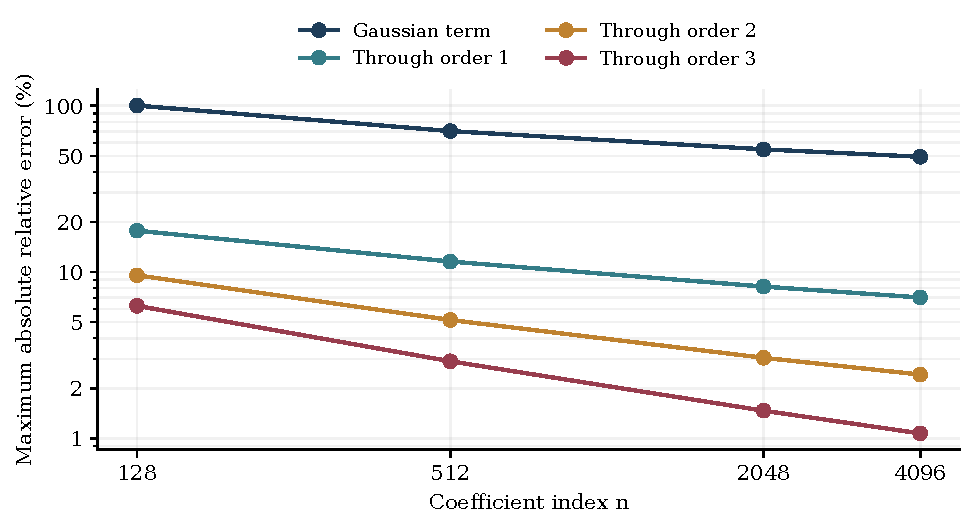
\includegraphics[width=0.91\textwidth]{figures/coefficient_refinement.pdf}
\caption{The errors in Table~\ref{tab:errors}, computed from finite
positive recurrences. The lines connect the four evaluated values of
$n$ and do not represent fitted convergence rates.}
\label{fig:refinement}
\end{figure}

The symbolic program verifies six total-degree identities through
degree five in the exponential--Stirling expansion; 36 central
Gamma-jet identities; and the five identities
$D_j=Q_j(-\log2)$ for $0\le j\le4$. The two algebraic routes use,
respectively, reciprocal Gamma products and positive-half-integer
Gamma moments. Nine noninteger-order Fourier quadratures, at 80
digits, check the parabolic cylinder normalization with absolute
errors below $10^{-65}$. Separate Fourier checks cover the order
derivatives used in the coefficient diagnostics. These computations
are sensitive to the Fourier sign and to the imaginary part of
$\Log(-iy)$.

For the inverse endpoint results, nine high-precision inverse
calculations cover $m=2,3,4$ and three small deficits $y$; six
upper-bank evaluations cover $s=1.25,1.4$ and three small $u$.
They agree with the proved reciprocal expansions and the negative
cut-modulus increment. The exact classifications in
Theorem~\ref{thm:ramification} follow from analytic continuation and
the displayed expansions, not from those samples.

Figure~\ref{fig:transition} illustrates only the normalized two-term
expression in Theorem~\ref{thm:wing-lambert}. This distinction matters:
the figure is an illustration of the explicit analytic profile,
whereas Figure~\ref{fig:refinement} compares independently computed
coefficients with their approximations.

\begin{figure}[htbp]
\centering
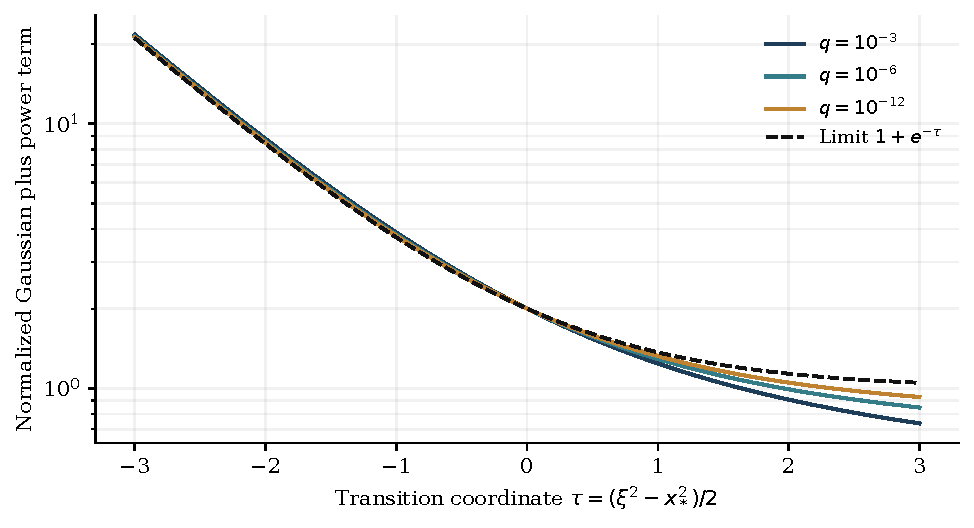
\includegraphics[width=0.91\textwidth]{figures/lambert_transition.pdf}
\caption{For $\xi=\sqrt{x_*(q)^2+2\tau}$, the exact normalized
two-term expression is
$e^{-\tau}+(1+2\tau/x_*(q)^2)^{-3/2}$.
The curves show this expression for three values of $q$ and its
limit $1+e^{-\tau}$. They are not sampled probabilities.}
\label{fig:transition}
\end{figure}
\FloatBarrier

\subsection{A focused audit and concrete proposed amendments}

No false printed theorem was established in the coefficient sources
used here. The useful corrections are statements of scope and
updates to explicit research questions. The accompanying
\mbox{\texttt{INTEGRATION.md}} gives proposed insertions without changing the
pinned repository. \path{THEOREM_LEDGER.md} records the hypotheses
and dependencies of each principal result. Source paths and hashes
are supplied in \path{PROVENANCE.json}.

\begin{enumerate}[label=\textbf{A\arabic*.},leftmargin=*]
\item \textbf{Mark the compact joint window of Q1 as resolved.}
Theorem~\ref{thm:all-orders} proves the requested joint coefficient
law, all fixed logarithmic corrections, and the uniform Fourier
bound. Equation~\eqref{eq:elementary-first} supplies the first
correction in the elementary scale requested there.
Equations~\eqref{eq:Lambert-scale}--\eqref{eq:matching} give the
exact marginal comparison. This is stronger than substituting
$s=s_n$ into a theorem whose constants were controlled only at
fixed $s$.

\item \textbf{Record a partial positive answer to Q2.}
Theorems~\ref{thm:positive-windows} and \ref{thm:wing-lambert}
give a relative approximation on every fixed polynomial window
in $\log n$, and an explicit transition profile. The negative
growing window and the passage to genuinely macroscopic
deviations remain open in this treatment.

\item \textbf{Retain the distinction between an endpoint value and
the coefficient radius.} The identity
$R_b^n a_n=\Prob(X_n=n)/n$ holds for every $b>0$.
The reference $R_b=e^{-(u-b)}$ is the actual radius on the
endpoint-controlled side $b\ge A$. For $b<A$, the principal
inverse encounters an interior fold and the radius is larger.
The uniform lattice estimate uses the reference value without
relabeling it as the radius below criticality.

\item \textbf{Add the reciprocal-order exception to endpoint
discussions.} The inverse endpoint is holomorphic at
$s=1+1/m$, $m\ge2$. An argument which treats every noninteger
polylogarithm branch point as a nonremovable inverse branch
point misses these exceptions. Theorem~\ref{thm:ramification}
gives the complete local replacement, with the minimal
ramification index. It makes no claim about other inverse
singularities at the same modulus.

\item \textbf{Qualify the proposed real-order extension of Q9.}
The cut-modulus inequality used for integer orders fails for
every $1<s<3/2$. Thus that proof cannot establish a blanket
real-order extension of the endpoint-circle statement in
\cite{repo-inverse}. This is a counterexample to the proposed
extension of the inequality, not to the existing integer theorem,
and it does not itself settle the global inverse Taylor radius.

\item \textbf{Keep the two convergence assertions separate.}
The implicit scale chart and the reciprocal-order inverse chart
are convergent holomorphic expansions. The coefficient series
is proved to every \emph{fixed} logarithmic order, with constants
depending on that order. Neither a convergent infinite Fourier
core expansion nor an optimal-truncation theorem is proved.
Uniform absolute error over all lattice points is also distinct
from a relative approximation where the probability vanishes.
The positive-window proof supplies the additional estimate in
exactly the range where it is used.
\end{enumerate}

\subsection{Further research questions with concrete starting points}

The following questions separate direct extensions from problems
requiring a different analytic mechanism. None is needed for the
validity of the results above.

\begin{enumerate}[label=\textbf{R\arabic*.},leftmargin=*]
\item \textbf{What is the relative law on growing negative
windows?} The Fourier theorem supplies an absolute error there,
but the algebraic positive tail is absent. A saddle displacement
on the negative side should be combined with the pole-paired
exponent before truncation. A useful first target is a relative
theorem for $-L^M\le\xi\le-r_L$, identifying the largest $M$
for which a finite expansion in the same parameters suffices.
This would address the remaining side of Q2 and quantify the
onset of the interior-fold regime.

\item \textbf{Can one join the compact resonance window to the
stable and finite-variance regions at every correction order?}
Here $|\lambda|$ is bounded. Letting $\lambda$ tend to either
infinity in the displayed formulas is not justified by this
proof. The leading all-rate results in \cite{repo-confluent}
suggest an overlap problem: construct uniform normalizations
and remainders when $\lambda=\lambda_n$ grows, then match to
fixed-order stable or finite-variance expansions. The exact
function $K_\eps$ is a natural common coordinate, but the
Fourier truncation and error constants must be redesigned.

\item \textbf{What is the first sector beyond all logarithmic
orders, and how does it remember the nonlinearity?}
The composition theorem removes all endpoint derivatives of
$G$ beyond the second from the fixed logarithmic sector.
Retain the cubic terms in
$G(\zeta(s)-D_s(t))$ and scale them by $nB^{-3}$.
This gives a concrete route to the first smaller sector,
including the first dependence on $G'''(\zeta(s))$.
The question is to prove a uniform mixed expansion in powers
of $B^{-1}$ and inverse logarithms, with a transparent
description of which endpoint derivatives first occur in
each sector.

\item \textbf{How fast do the coefficient functions grow with
the truncation order?} The finite formulas reduce this to
joint large-order estimates for Stirling numbers and
$\HH_{2k}^{[j]}$. Determine a useful Gevrey bound on compact
spatial sets, investigate optimal truncation, and identify the
associated exponentially small remainder. Any summation
procedure must respect the Fourier tail: the untruncated
exponential obtained from the local model need not be
integrable on the full real line. Formal exponentiation
alone therefore cannot supply this result.

\item \textbf{How far can the relative positive window be
extended?} The present argument reaches $\xi\le L^M$ for
every fixed $M$, by choosing a sufficiently large but fixed
logarithmic order. For displacements of algebraic size in
$n$, this argument loses relative control. A direct uniform
local large-deviation estimate for the triangular compound
Poisson family could bridge the gap to fixed supercritical
$b>A$, while keeping the exact amplitude
$b^{s-1}(b-A)^{-s}$. The work of \cite{berger} is an
appropriate starting point for the required probability
estimates, with the moving-law uniformity proved explicitly.

\item \textbf{What determines the global inverse radius at a
removable reciprocal endpoint?} Local removal of the value
$\zeta(1+1/m)$ does not locate the next singularity of the
inverse germ. Determine which critical values, asymptotic
values, or sheet obstructions first meet its continuation.
Potential critical points away from zero satisfy
$\Li_{1/m}(z)=0$. Even the case $m=2$ would clarify whether
other singularities can retain the endpoint modulus after
the positive endpoint itself becomes removable.

\item \textbf{Can order jets and ramification be organized
uniformly in the jet index?} The convergent reciprocal chart
handles every fixed jet and compact $\tau$.
The leading term shows that differentiation in order restores
logarithms despite local removability at the central order.
Determine the allowable joint growth of the derivative
index, $|\log y|$, and the winding number. This would connect
the exact monodromy and order-jet calculus of the existing
Polylogarithms chapters with quantitative inverse estimates.

\item \textbf{What is the sharp positivity hypothesis for
composition universality?} The sufficient condition
$G'(0)>0$ gives a uniform coefficient lower bound and
aperiodicity immediately. Some positive outer functions
with $G'(0)=0$ may still have the needed tail mass and
lattice span after composition. Characterize the weakest
conditions that yield the two Fourier bounds, and then
separate these probabilistic conditions from the local
analytic conditions at $\zeta(s)$.

\item \textbf{Can several colliding tail terms be treated by
one finite calculus?} Replace a single polylogarithm by a
positive combination with orders moving through the same
integer, or add controlled slowly varying factors obtained
by order differentiation. The scalar divided difference
suggests a multivariate Stirling or Bell-polynomial
description. The challenge is to choose a normalization
that preserves uniform positivity and keeps all pole
cancellations explicit.

\item \textbf{Which part should be formalized first?}
A tractable initial layer consists of the finite
coefficient--probability identity, the Gamma recurrence
pairing, the Stirling coefficient formula, and the
reciprocal-order Lagrange identities. The analytic layer
then needs parameter-uniform Fourier inversion,
dominated convergence with logarithmic powers, and
holomorphic implicit inversion. This separation would
produce reusable formal components rather than a
single opaque formalization of the final theorem.
\end{enumerate}

The central structural point is that the collision at $s=3$ can be
absorbed into an exact scale while leaving a finite order-derivative
calculus for every correction. Positivity provides the global Fourier
control needed to turn that local calculus into a theorem. The
reciprocal inverse endpoints exhibit the complementary phenomenon:
ramification can disappear at an exceptional order, while its
logarithmic dependence remains visible to differentiation in order.

\clearpage
\begin{thebibliography}{99}
\addcontentsline{toc}{section}{References}

\bibitem{repo-boundary}
ProveIt research collection.
\emph{Boundary Completion for Quadratic Polylogarithm Feedback:
Convergent inverse transseries, logarithmic resonance, and coefficient
transitions}. 12 October 2026.
\href{https://github.com/VladimirReshetnikov/ProveIt/tree/8f5afd4d7565df808359f6a0c22f87f79a119bb9/Analysis/Transseries/docs/series-and-transseries/Quadratic_Polylogarithm_Feedback_Boundary_Completion}{Pinned report and sources}.
In particular, Sections 5--7: the joint inverse chart, fixed-order
coefficient theorem, and research questions Q1--Q2.

\bibitem{repo-gaussian}
ProveIt research collection.
\emph{Through the Stable--Gaussian Endpoint:
Uniform critical transseries, prefix-independent cutoff corrections,
and conditional extremes}. 29 September 2026.
\href{https://github.com/VladimirReshetnikov/ProveIt/blob/8f5afd4d7565df808359f6a0c22f87f79a119bb9/Analysis/Transseries/docs/series-and-transseries/Stable_Gaussian_Endpoint_Uniform_Critical_Transseries/article.tex}{Pinned article source}.

\bibitem{repo-confluent}
ProveIt research collection.
\emph{Confluent Critical Transseries Across the Exponent-Two Boundary:
A Uniform Inverse Chart, Conditional Poisson Limits, and Sharp
Action Budgets}. 29 September 2026.
\href{https://github.com/VladimirReshetnikov/ProveIt/blob/8f5afd4d7565df808359f6a0c22f87f79a119bb9/Analysis/Transseries/docs/series-and-transseries/Confluent_Critical_Transseries_Exponent_Two_Boundary/Confluent_Critical_Transseries.tex}{Pinned article source}.

\bibitem{repo-marginal}
ProveIt research collection.
\emph{Marginal Critical Transseries:
Convergent Lambert--W Charts, Universal Cutoff Corrections,
and Certified Action Budgets}. 29 September 2026.
\href{https://github.com/VladimirReshetnikov/ProveIt/blob/8f5afd4d7565df808359f6a0c22f87f79a119bb9/Analysis/Transseries/docs/series-and-transseries/Marginal_Critical_Transseries_Action_Budgets/Marginal_Critical_Transseries.tex}{Pinned article source}.

\bibitem{repo-moments}
ProveIt collective Polylogarithms manuscript.
\emph{Lambert inversion and exact logarithmic coefficients}.
Integrated chapter \path{01-lambert-moments.tex}, at the inspected
12 October 2026 snapshot.
\href{https://github.com/VladimirReshetnikov/ProveIt/blob/8f5afd4d7565df808359f6a0c22f87f79a119bb9/Analysis/Polylogarithms/docs/manuscript/chapters/01-lambert-moments.tex}{Pinned chapter source}.

\bibitem{repo-inverse}
ProveIt research collection.
\emph{Resonant Order Jets and Convergent Inverse Transseries:
for Polylogarithms and Logarithmically Weighted Tails}.
12 October 2026.
\href{https://github.com/VladimirReshetnikov/ProveIt/blob/8f5afd4d7565df808359f6a0c22f87f79a119bb9/Analysis/Transseries/docs/series-and-transseries/Polylogarithm_Resonance_And_Inverse_Transseries/polylogarithm_resonance_and_inverse_transseries.tex}{Pinned article source}.
In particular, the noninteger inverse charts and research question 9,
``Global geometry beyond integer orders.''

\bibitem{dlmf-polylog}
NIST Digital Library of Mathematical Functions.
\emph{\S25.12, Polylogarithms}, especially formula 25.12.12.
\url{https://dlmf.nist.gov/25.12}.
Accessed 12 October 2026.

\bibitem{dlmf-cylinder}
NIST Digital Library of Mathematical Functions.
\emph{Chapter 12, Parabolic Cylinder Functions}:
\href{https://dlmf.nist.gov/12.2}{\S12.2, definitions and initial values};
\href{https://dlmf.nist.gov/12.5}{\S12.5, integral representations,
especially formula 12.5.4};
\href{https://dlmf.nist.gov/12.9}{\S12.9, large-variable asymptotic expansions}.
Accessed 12 October 2026.

\bibitem{dlmf-lambert}
NIST Digital Library of Mathematical Functions.
\emph{\S4.13, Lambert $W$-Function}.
\url{https://dlmf.nist.gov/4.13}.
Accessed 12 October 2026.

\bibitem{lam}
H. Lam, J. Blanchet, D. Burch, and M. Z. Bazant.
Corrections to the Central Limit Theorem for Heavy-tailed Probability
Densities.
\emph{Journal of Theoretical Probability} \textbf{24}(4) (2011),
895--927.
\href{https://doi.org/10.1007/s10959-011-0379-y}{doi:10.1007/s10959-011-0379-y}.
\href{https://www.columbia.edu/~khl2114/files/LBBB.pdf}{Author-hosted final text}.

\bibitem{berger}
Q. Berger, M. Birkner, and L. Yuan.
Collective vs. individual behaviour for sums of i.i.d. random variables:
appearance of the one-big-jump phenomenon.
\emph{Annales de la Facult\'e des Sciences de Toulouse}, Series 6,
\textbf{33}(5) (2024), 1413--1485; published online 24 April 2025.
\href{https://afst.centre-mersenne.org/articles/10.5802/afst.1802/}{doi:10.5802/afst.1802}.

\end{thebibliography}

\end{document}
